\chapter{TDT4295 - Computer Design Project}
\label{sec:intro}

The Computer Design Project is held at NTNU every fall.
It is a large, project-based subject in which students create a working computing platform, more or less from scratch.
This year saw high enough participation that two assignments were presented, and two groups formed around these.
The report you're now reading details the work done and solution implemented by the vector graphics processor group.

This chapter introduces the project, describes the requirements, outlines the solution and provides a fundamental understanding of vector graphics. It ends with an introduction of the labs that were used and a general overview of the whole report.

\section{Assignment}

This year's assignment focuses on graphics, exploring both of the traditional ways of representing and processing graphics: raster-based and vector-based.
Two distinct assignment texts were presented by the course staff: one focusing on raster-based graphics, the other on vector graphics.
The following is a verbatim copy of the vector graphics assignment text \cite{assignment-text}.

\subsection{Assignment Text - A Vector Graphics Processor}

Image generation using vector graphics as the core method is a powerful and scalable way of generating image data.
Vector graphics represents images at a higher abstraction level than single-pixels.
A vector graphics processor can make use of drawing instructions to produce images, which is a task well suited for hardware acceleration \cite{openvg}.
Parallelization with multiple cores and/or at the instruction level are architectural possibilities that can be exploited to design a specialized processor.
The task is to design and implement a processor for producing vector graphics.
Figure \ref{fig:vector-display-network-analyzer} illustrates a vector display which takes in vector drawing commands (instead of a stream of pixels) as input.

\begin{figure}[h!]
    \centering
    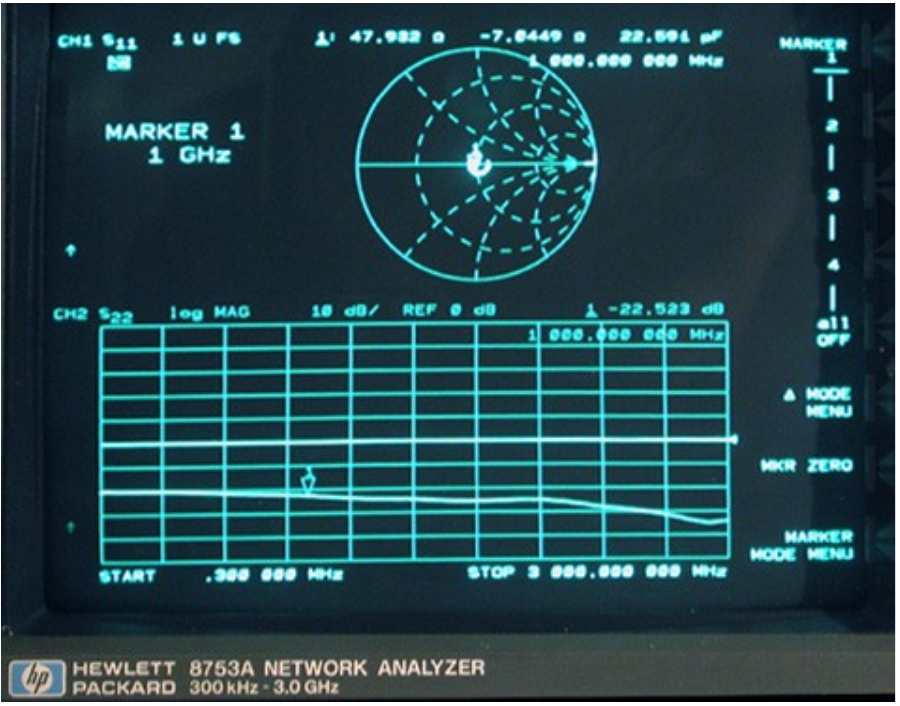
\includegraphics[width=0.6\linewidth]{images/network-analyzer-vector-graphics-display.png}
    \caption{A vector graphics display on a network analyzer\cite{assignment-text}.}
    \label{fig:vector-display-network-analyzer}
\end{figure}

\section{Vector Graphics - A Short Introduction}
Vector graphics expresses the contents of an image by using primitives, which are defined mathematically.
Primitives can be objects like lines (defined by their endpoints), squares (defined as a bounding box of two points) or curves (defined by the position of control points).
One particular kind of curves, called bézier curves, can be used to define complex, vectorized shapes.
The points are relative to the coordinate system of a 'scene', which is an abstract representation of an image.
Scenes are not tied to any specific physical screen resolution, but can be scaled to fit any resolution without loss of detail.

The major advantages of vector graphics are expressiveness and scalability.
Modern computing devices come in many sizes and aspect ratios.
With raster based solutions, graphics have to be regenerated for each new display size.
A vector based solution is inherently resolution independent, allowing for asset reuse across devices.

More information about vector and raster graphics is found in Chapter \ref{chp:background}.

\section{Requirements}
\label{sec:requirements}
The group decided on a set of functional requirements based on initial research, listed in Table \ref{tbl:func_req}.
Non-functional requirements given in the assignment text are listed in Table \ref{tbl:non_func_req}.

\begin{table}[h!]
\resizebox{\textwidth}{!}{
    \begin{tabular}{|l|l|}
        \hline
        \textbf{Requirement}                                                    & \textbf{Priority} \\ \hline
        The system should be able to produce and process vector primitives      & High     \\ \hline
        The system should display primitives on a vector display               & High     \\ \hline
        The system should support both straight lines and general bézier curves & High     \\ \hline
        The processor should be general                                         & High     \\ \hline
        The system should support modification of primitives                    & Medium   \\ \hline
        The system should rasterise primitives and support HDMI as an output    & Medium   \\ \hline
        A toolchain supporting the system should be available                   & Low      \\ \hline
    \end{tabular}
}
    \caption{Functional requirements.}
    \label{tbl:func_req}
\end{table}


\begin{table}[h!]
\resizebox{\textwidth}{!}{
    \begin{tabular}{|l|l|}
     	\hline
        \textbf{Requirement}    												& \textbf{Priority} \\ \hline
        The processor should be implemented on a Xilinx \gls{fpga}								& High 	\\ \hline
        The unit must utilize a Silicon Labs EFM32 microcontroller to act as an				& High 	\\
        \gls{io} processor 																		&   	\\ \hline
        The budget of 10 000 NOK should cover components and \gls{pcb} production					& Medium 	\\ \hline

    \end{tabular}
}
    \caption{Non-functional requirements.}
    \label{tbl:non_func_req}
\end{table}


\section{A Vector Graphics Computer Architecture}

\begin{figure}[H]
    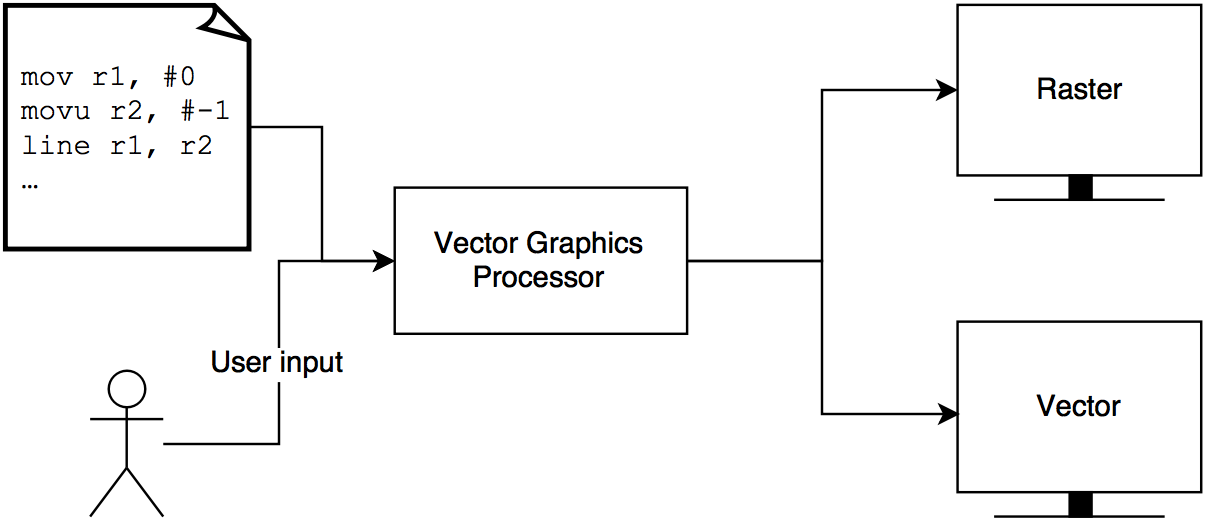
\includegraphics[width=\linewidth]{images/high_level_io.png}
    \caption{\gls{io} overview.}
    \label{fig:io-overview}
\end{figure}

Based on the requirements, the group chose to make a general purpose computer with support for producing and processing vector graphics.
The computer would read instructions from memory, execute them on a processor core, and render vector based scenes to different outputs.
To showcase the nature of vector graphics, a vector display in the form of an oscilloscope was chosen as the primary output device.
HDMI was included as secondary output to a raster display.
As a whole, the system should be assembled on a custom PCB, with the microcontroller serving as an \gls{io}-unit while the main processor architecture and output-modules should be implemented on the \gls{fpga}.

\section{Lab Environment}
The NTNU Computer Design Lab was used frequently for this project.
The lab contains a wide variety of oscillators, signal generators and logic analyzers, which was used to test different parts of the system.
The lab also contains soldering equipment and aids - which were used extensively by the team when soldering the \gls{pcb} - as well as a lot of assorted electronic components.

A second lab at NTNU, ITV-458, was used by the team when programming the solution.
The lab contains computers running Ubuntu and tools for working with \gls{fpga}s.

\section{About this report}
This report is meant to give a thorough understanding of the system designed by the group.
Having introduced the assignment and described a very abstracted architecture, the next chapters introduces the system created by the group, as well as they give some background on computer graphics and a theoretical overview of vector graphics.

Part two presents the designed architecture in detail, outlines the programming model and elaborates on the implementation of specific subparts of the system.

Finally, part three presents performed tests, results, discussion and a conclusion.

It should be noted that in this report, 'the group' refers to everyone working on this project. The main work loads (System architecture, \gls{io} and \gls{pcb} design), were split among smaller teams. 'The team' refers to the team responsible for this functionality.
